\documentclass[10pt,conference]{IEEEtran}

% A self-contained, early research draft for Overleaf.
\usepackage{amsmath,amssymb}
\usepackage{graphicx}
\usepackage{booktabs}
\usepackage{cite}
\usepackage{tikz}
\usepackage{placeins}


\usetikzlibrary{arrows.meta,positioning,shapes.geometric,calc}

\tikzset{
  pbox/.style={
    draw,
    rounded corners=2pt,
    align=center,
    text width=2.65cm,
    minimum height=9mm,
    inner sep=3pt,
    font=\footnotesize
  },
  pwide/.style={
    pbox,
    text width=3.05cm
  },
  pdecision/.style={
    draw,
    diamond,
    aspect=2,
    align=center,
    text width=1.35cm,
    inner sep=1pt,
    font=\scriptsize
  },
  pedge/.style={
    -{Stealth[length=2mm]},
    line width=0.6pt
  },
  plabel/.style={
    fill=white,
    inner sep=1.5pt,
    font=\scriptsize
  },
  pplanned/.style={
    pbox,
    dashed
  }
}

\usepackage{algorithm}
\usepackage{algpseudocode}

% Authorization decision labels

\newcommand{\Allow}{\ensuremath{\mathrm{ALLOW}}}
\newcommand{\Ask}{\ensuremath{\mathrm{ASK}}}
\newcommand{\Block}{\ensuremath{\mathrm{BLOCK}}}
\newcommand{\Pass}{\ensuremath{\mathrm{PASS}}}
\newcommand{\Deny}{\ensuremath{\mathrm{DENY}}}


\usepackage[hidelinks]{hyperref}
\raggedbottom

\begin{document}

\title{Policy-Bounded Authorization and Approval Learning for Tool-Using LLM Agents}

\author{
\IEEEauthorblockN{Siddharth Magesh}
\IEEEauthorblockA{University of Southern California\\
Los Angeles, CA, USA\\
\href{mailto:smagesh@usc.edu}{smagesh@usc.edu}}
\and
\IEEEauthorblockN{Atharva Thorat}
\IEEEauthorblockA{University of Southern California\\
Los Angeles, CA, USA\\
\href{mailto:atharvas@usc.edu}{atharvas@usc.edu}}
\and
\IEEEauthorblockN{Kaustubh Adhe}
\IEEEauthorblockA{University of Southern California\\
Los Angeles, CA, USA\\
\href{mailto:adhe@usc.edu}{adhe@usc.edu}}
}

\maketitle

\begin{abstract}
The increasing adoption of autonomous AI agents in digital workspaces introduces a fundamental challenge: ensuring that agents operate within the scope of authority granted by their users while retaining the flexibility required to perform diverse tasks. Existing authorization approaches often rely on static permission policies or repeated evaluations by general-purpose language models. Static policies can be restrictive and difficult to adapt to changing task requirements, while model-based evaluations introduce computational overhead and may be susceptible to prompt injection and unintended authorization decisions. Furthermore, systems that learn from repeated user approvals risk permission creep, where individually accepted actions gradually expand an agent's effective authority beyond the user's original intentions.

\vspace{5pt}


This paper presents a policy-bounded authorization
framework that separates deterministic permission
enforcement, contextual action assessment, and
user-specific approval learning. The framework
combines an external enforcement layer with a
lightweight decision model that evaluates proposed
tool actions against the authentic user request
and verified contextual evidence. Persistent
exact-action grants and a bounded contextual
learner support permission reuse without
independently expanding the underlying policy.

We evaluate three permission configurations
using 36 constructed action sequences, with
504 action checks per configuration. Explicit
grants reduce confirmation requests by 17.26\%,
while active contextual learning achieves a
5.36\% reduction relative to the no-memory
baseline. All configurations record zero
forbidden dispatches under the scenario oracle.
Separate Laya evaluations reveal limitations
in authorization classification against
provisional labels. These findings demonstrate
the feasibility of policy-bounded permission
reuse while identifying the need for improved
contextual learning and model validation.


\end{abstract}

\vspace{5pt}
\begin{IEEEkeywords}
Policy-Bounded Learning, Runtime Authorization,
Contextual Action Validation, Approval-Conditioned
Adaptation, Dynamic Privilege Management,
Authorization Drift, Lightweight Decision Models
\end{IEEEkeywords}

\section{Introduction}
Large language model (LLM) agents are increasingly being integrated into digital workspaces, software development environments, and enterprise applications, where they interact with external systems through tools and APIs. Unlike conventional language models that primarily generate textual responses, these agents perform tasks through sequences of actions, including reading files, executing commands, accessing databases, modifying resources, and communicating with external services. A single user request may require numerous tool invocations, with each action depending on the information retrieved and decisions made during earlier steps. Consequently, authorization cannot be treated as a one-time decision made when a task begins. Each proposed tool action must be evaluated against the user's original intent, the current execution context, and the permissions applicable to that particular operation.

This requirement introduces a significant security challenge. Although an agent may be granted access to a collection of tools, that access does not imply authorization to use every available capability for every task. For example, a software development agent may be permitted to inspect a repository, execute tests, and modify source files. However, the same task does not automatically authorize it to access credentials, modify unrelated configurations, execute destructive commands, or transmit repository contents to an external service. These distinctions become increasingly difficult to maintain during long-running tasks, where the agent continuously processes new information and generates subsequent tool calls. An action that appears reasonable in isolation may exceed the user's intended authorization when considered in the context of the complete task.

Prompt injection further complicates this problem. Instructions embedded in emails, documents, repository files, web pages, and other tool outputs can influence an agent's subsequent actions, potentially redirecting its execution toward objectives that were never authorized by the user. Since agents repeatedly incorporate external observations into their planning and tool-selection processes, an instruction encountered during one stage can influence actions several steps later. AgentDojo \cite{debenedetti2024agentdojo} provides a dynamic environment for studying this problem by evaluating agents on stateful tasks involving external tools and untrusted data. Its benchmark combines legitimate user objectives with attacker-controlled instructions and evaluates both task utility and attack success. Importantly, AgentDojo demonstrates why agent security must be considered across complete execution trajectories rather than through isolated prompt or response classification.

A natural approach to mitigating these risks is to introduce permission enforcement between the agent and its external tools. Deterministic authorization policies can restrict tool access and constrain arguments, recipients, resources, and other action parameters. However, a single static permission configuration may not adequately represent the changing requirements of different tasks. Policies that are too restrictive can prevent legitimate multi-step workflows from completing, whereas broadly defined permissions can allow unnecessary or unintended actions. Furthermore, restrictions expressed only through system instructions or natural-language prompts do not constitute independent enforcement. An agent influenced by untrusted information may still propose an action that contradicts those instructions. Security therefore requires an external mechanism that evaluates proposed actions at the tool-execution boundary and prevents unauthorized operations from reaching the underlying environment.

Existing research has begun addressing this challenge through runtime privilege control. Progent \cite{shi2025progent}, for example, introduces a programmable policy mechanism that generates and updates task-specific privileges as execution progresses. Its use of symbolic policy representations and an SMT-based verification procedure distinguishes permission expansion from permission restriction. Restrictions can be applied automatically, while expansions require explicit approval, establishing a monotonic confinement property that prevents silent privilege escalation. This provides an important foundation for dynamic authorization. However, the broader design space still raises questions about the computational cost of repeated policy evaluation, the use of lightweight decision models for contextual action assessment, and how authorization preferences can be learned across repeated interactions without unintentionally transferring permissions between tasks or resources.

One practical consideration is the computational overhead associated with evaluating every proposed action. Long-running agent workflows may involve numerous tool calls, and repeatedly invoking a general-purpose generative model to inspect each action can introduce additional inference costs and latency. This becomes particularly relevant when the evaluation requires reasoning about the relationship between the user's request, the proposed operation, and the surrounding execution context. We therefore investigate the use of lightweight, System-1-style decision models as an alternative for action-level authorization. Rather than generating unrestricted natural-language evaluations, these models produce structured decisions and associated probability estimates. The intended approach is to evaluate every proposed tool invocation before execution, using the authentic user request, the proposed action, and relevant verified context. This places the authorization check at the point where an action produces an external effect, without requiring access to the agent's private internal reasoning. It also creates an opportunity to investigate whether specialized decision inference can reduce computational overhead while maintaining sufficient decision quality.

Beyond action-level enforcement, authorization systems must also account for how permissions evolve through repeated user interactions. When an agent encounters an action that requires confirmation, the user's response provides information about their preferences and expectations. However, repeatedly accepting similar actions does not necessarily imply that the user intends to authorize them permanently or across unrelated tasks. For example, approving a file modification within one repository should not automatically authorize modifications across all repositories. Similarly, permission to communicate with a particular contact for one task should not become unrestricted permission to communicate with that contact in every future context. Systems that generalize individual approvals without preserving their original scope can gradually expand an agent's effective authority. We refer to this unintended expansion as permission creep. Persistent authorization memories introduce an additional concern: permissions learned in one task or execution context may become stale or be incorrectly reused in another. Effective permission learning must therefore preserve the relationship between an approval, its originating task, the affected resource, and the applicable policy.

To address these challenges, we propose a policy-bounded authorization framework that separates deterministic enforcement, contextual action assessment, and adaptive permission management. The framework introduces an external permission boundary that defines the maximum authority available to the agent. Within this boundary, a lightweight decision-model Gatekeeper evaluates proposed tool actions and produces one of three decisions: ALLOW, ASK, or BLOCK. Actions that violate explicit policy restrictions are rejected independently of the model's prediction, while uncertain actions can be referred to the user for confirmation. An approval-learning component subsequently uses user feedback to reduce unnecessary interruptions. We investigate both repeated-approval counting and explicit, scoped authorization grants, with the latter requiring deliberate user authorization before a permission can be reused. Dynamic permission scoping, policy-version checks, expiration, and revocation are considered to limit unintended permission transfer across tasks and execution contexts. We further identify feedback-driven adaptation of the decision model itself as a potential extension, in which verified approval data may be used to update model parameters without weakening the external permission boundary.


This work investigates whether policy-bounded
authorization can support adaptive permission
reuse without weakening independently enforced
security constraints. We implement a deterministic
enforcement boundary, a lightweight contextual
Gatekeeper, persistent exact-action grants, and
a user-specific contextual learner.

We evaluate the implemented components through
controlled permission sequences, offline
Gatekeeper comparisons, and a limited real-model
integration check. The experiments examine
authorization enforcement, confirmation
reduction, and the behavior of adaptive
permission reuse. Full AgentDojo evaluation
and periodic model fine-tuning remain subjects
of subsequent investigation.


% ==========================================
% II. BACKGROUND AND RELATED WORK
% ==========================================

\section{Background and Related Work}

\subsection{Authorization in Tool-Using LLM Agents}

Large language model agents interact with external environments through tools that provide access to files, applications, databases, and other resources. These interactions introduce authorization requirements that extend beyond conventional access control. Traditional Role-Based Access Control (RBAC) and Attribute-Based Access Control (ABAC) determine whether a principal can perform an operation on a resource based on assigned roles, attributes, and applicable policies. However, tool-using agents operate through sequences of actions whose necessity and authorization depend on the user's current objective and the state of the execution environment.

Consequently, permission to access a tool does not necessarily imply permission to perform every operation exposed by that tool. An agent authorized to access an email service, for example, may need to read messages for one task and send a response for another. The authorization requirements differ even though both operations use the same service. This distinction becomes particularly important in multi-step workflows, where an agent's subsequent actions depend on information obtained from previous tool calls. Each proposed action must therefore be evaluated against the original user request, its intended effects, and the relevant execution context before it is allowed to proceed.

This motivates task-conditioned authorization and least-privilege enforcement for autonomous agents. Rather than granting unrestricted access to available tools, an authorization mechanism should constrain each action to the authority necessary for the current task. Such enforcement should operate independently of the agent's natural-language reasoning so that instructions encountered in untrusted content cannot directly modify the permissions governing tool execution.

\subsection{Runtime Policy Enforcement and Contextual Authorization}

Recent research has explored external policy enforcement as a means of controlling the actions of tool-using agents. Progent introduces a programmable privilege-control framework in which policies describe permitted tool calls and their arguments using a domain-specific language \cite{shi2025progent}. These policies are enforced deterministically outside the agent. Progent also supports dynamic policy generation and updates through an LLM, with an SMT-based verification mechanism that distinguishes permission restrictions from expansions. Restrictive updates can be applied automatically, whereas expansions require explicit user approval. This establishes a monotonic confinement property that prevents unapproved privilege expansion.

Conseca addresses the relationship between an action and the context in which it is performed \cite{tsai2025conseca}. It proposes generating just-in-time security policies from the user's request and trusted contextual information. The resulting policies define which actions are appropriate for a particular purpose and are enforced deterministically. This work demonstrates the importance of contextual authorization rather than relying exclusively on globally defined permissions. Its primary focus, however, is the generation and enforcement of contextual policies rather than learning individualized authorization decisions from accumulated user feedback.

MiniScope further investigates least-privilege authorization through a hierarchical permission model \cite{zhu2025miniscope}. It reconstructs relationships between tool permissions using service authorization scopes or historical tool-use traces, allowing related capabilities to be grouped into task-level roles. Its two-layer permission mechanism aims to reduce repeated tool-level confirmation requests while preserving explicit authorization boundaries. MiniScope is particularly relevant to the usability challenges of agent permissions, as it demonstrates that authorization granularity directly affects both security and user interaction overhead. Its security guarantee is defined relative to the permission hierarchy: it prevents execution outside delegated permissions, but does not determine whether an action is appropriate when it already falls within an authorized role.

Together, these systems establish important foundations for external enforcement, contextual policies, and task-scoped permissions. They also illustrate that authorization must account for both the capabilities available to an agent and the purpose for which those capabilities are being used.

\subsection{Task-Conditioned Least Privilege and Behavioral Constraints}

Another direction investigates whether an agent's behavior can be constrained using task-specific execution requirements and learned behavioral boundaries. Agent-Sentry constructs behavioral bounds from recurring agent functionalities and their execution traces \cite{sequeira2026agentsentry}. It learns policies from these traces and blocks tool calls that deviate from the established behavior or conflict with the user's intended task. This approach provides a means of identifying actions that fall outside expected execution patterns, although its effectiveness depends on the quality and coverage of the learned behavioral bounds.

Task-Conditioned Least-Privilege Learning investigates model-level adaptation through offline post-training \cite{tu2026tasklp}. It defines task-specific sufficient-authority envelopes and uses deterministic auditing of agent actions and their observed effects to guide training. The objective is to teach an agent to complete tasks without exercising unnecessary authority. Unlike runtime permission systems that primarily intercept proposed actions, this approach attempts to improve the agent's own selection of task-appropriate actions through model training. It provides a relevant precedent for learning-based least-privilege behavior, while retaining external auditing as an additional security mechanism.

SkillScope addresses over-privileged behavior in reusable Agent Skills through graph-based analysis of natural-language instructions and executable operations \cite{wu2026skillscope}. It identifies actions that exceed the scope of a user's current task, validates their necessity, and constrains their execution through task-conditioned control-flow modifications. This demonstrates that excessive authority can originate not only from individual tool calls but also from the procedures and reusable capabilities through which agents execute tasks.

These approaches establish that task-specific authority and learned behavioral constraints are important components of agent security. However, they primarily investigate policy enforcement, behavioral restriction, or offline model adaptation. Our research additionally investigates how authorization decisions can adapt to individual users through explicit approval feedback while remaining within independently enforced permission boundaries.

\subsection{Prompt Injection and Multi-Step Agent Evaluation}

Prompt injection presents a particular challenge for agents that interact with untrusted external content. Instructions embedded in retrieved documents, emails, web pages, or tool responses may influence subsequent agent actions and redirect execution away from the original user objective. Since agent workflows involve multiple dependent tool calls, an injected instruction encountered during an intermediate step may affect later operations rather than producing an immediately identifiable malicious action.

AgentDojo provides a dynamic evaluation environment for studying prompt-injection attacks and defenses in tool-using LLM agents \cite{debenedetti2024agentdojo}. It includes 97 realistic tasks and 629 security test cases across application environments such as email management, e-banking, and travel booking. The benchmark evaluates agent utility and security under interactions with untrusted data and supports the evaluation of different attack and defense strategies.

AgentDojo is particularly relevant to our work because it provides stateful tasks in which security decisions must remain consistent across multiple tool interactions. However, it is an evaluation framework rather than an authorization mechanism. Its task-completion and attack-success measurements do not, by themselves, establish whether an individual tool action was correctly classified as permitted, confirmation-required, or prohibited. We therefore consider action-level authorization accuracy, confirmation frequency, and permission-scope changes as complementary evaluation measures.

\subsection{Feedback-Driven Adaptation and Continual Learning}

Learning from user feedback provides another direction for improving the behavior of autonomous agents. Contextual bandit algorithms offer a general framework for adapting decisions using contextual information and observed feedback. For example, Li et al. introduced a contextual-bandit approach for personalized recommendation, demonstrating how a decision policy can adapt to individual users through sequential interaction \cite{li2010contextualbandit}. Algorithms such as LinUCB and Thompson Sampling provide possible approaches for learning personalized decision policies without requiring continuous modification of a large underlying model.

In the authorization setting, such methods could be investigated to adapt confirmation decisions using action characteristics, model predictions, and user-specific interaction history. However, user approval is not equivalent to proof that an action should have been automatically authorized. An approval applies to the action presented to the user and should not independently establish broader permissions. Consequently, feedback-driven adaptation must operate within explicit authorization scopes rather than treating repeated approvals as unrestricted permission grants.

Model-level adaptation provides a complementary direction. Task-Conditioned Least-Privilege Learning \cite{tu2026tasklp} demonstrates the use of offline post-training to improve task-conditioned authority selection. Continual-learning research also highlights the importance of preserving useful knowledge while avoiding interference between unrelated tasks. AgentCL investigates the evaluation of reusable experience across controlled task streams \cite{shu2026agentcl}, while ConsistencyGate examines the propagation of unreliable information through persistent agent memory \cite{zhang2026consistencygate}. Although these studies do not directly address permission authorization, they motivate careful handling of feedback, memory isolation, and cross-task information reuse.

Building on these directions, we investigate two complementary forms of adaptation: per-user online learning of authorization decisions and periodic fine-tuning of a lightweight decision model using verified feedback. These mechanisms are considered separately from the external permission policy. In particular, learned preferences must not override explicit restrictions, and approval information must retain its original user, task, resource, and policy scope.

\subsection{Research Positioning}

Existing research has established several important approaches to securing tool-using agents, including deterministic privilege enforcement, dynamically generated contextual policies, hierarchical permission models, behavioral constraints, and task-conditioned model training. Progent demonstrates how policy updates can be formally checked before being applied, while MiniScope shows how hierarchical permissions can reduce repeated confirmation requests without abandoning explicit authorization. Agent-Sentry and SkillScope investigate behavioral and task-specific restrictions, and Task-Conditioned Least-Privilege Learning demonstrates that model training can improve an agent's selection of necessary authority.

Our work builds on these foundations and investigates a complementary problem: how to adapt action-level authorization decisions from user feedback without allowing the learning process to expand the authority established by an external policy. Specifically, we examine the use of a lightweight decision model to evaluate proposed tool actions, explicit scoped permissions to represent reusable user authorization, and contextual learning to adapt confirmation behavior for individual users. Periodic fine-tuning of the decision model is considered as a further means of improving its general authorization judgments using verified feedback.

The distinction is between adapting authorization decisions and changing the underlying security policy. Our proposed approach seeks to improve the former while keeping the latter independently enforced. This provides the basis for evaluating whether user-specific adaptation can reduce unnecessary confirmation requests and computational overhead without increasing unauthorized actions or transferring permissions across unrelated execution contexts.



% ==========================================
% III. PROBLEM FORMULATION AND THREAT MODEL
% ==========================================

\section{Problem Formulation and Threat Model}

\subsection{System Model}

We consider a tool-using LLM agent operating on behalf of an authenticated user $i$, who initiates a task through an original request $r_i$. During execution, the agent interacts with external tools and generates a sequence of proposed actions. Let the execution history at step $t$ be denoted by $H_t$, containing the previous actions and their corresponding observations. Based on this history, the agent proposes a new action:

\begin{equation}
a_t = (\tau_t, \mathbf{v}_t, \rho_t, e_t),
\end{equation}

where $\tau_t$ represents the selected tool, $\mathbf{v}_t$ denotes its arguments, $\rho_t$ identifies the target resource, and $e_t$ represents the expected action effects.

The agent operates under a versioned user-defined permission policy $P_i^{(v)}$. The execution environment also provides trusted contextual information $c_t$, including resource identities, tool metadata, and relevant state information. Observations obtained from external sources may contain untrusted content $z_t$, which can influence subsequent agent actions but cannot independently establish authorization.

The authorization mechanism evaluates each proposed action before it reaches the corresponding tool. The decision input is represented as:

\begin{equation}
x_t = (r_i, a_t, c_t, z_t, P_i^{(v)}).
\end{equation}

This formulation treats authorization as a sequential decision problem rather than a one-time permission check. Each action is evaluated against the original user request and the current execution state, including actions proposed after intermediate tool observations.

\subsection{Authorization Decision Problem}

The authorization problem consists of determining whether a proposed action is permitted by the user's policy, justified by the current task, and sufficiently supported by available evidence.

First, a deterministic policy evaluator computes:

\begin{equation}
W(P_i^{(v)},a_t,c_t)
\in \{\mathrm{PASS},\mathrm{DENY}\}.
\end{equation}

An action receiving $\mathrm{DENY}$ cannot proceed to execution, regardless of subsequent model predictions or learned preferences.

For actions that pass this check, the contextual Gatekeeper estimates a probability distribution over three authorization decisions:

\begin{equation}
p_{\theta}(y \mid x_t),
\qquad
y \in \mathcal{Y},
\end{equation}

where:

\begin{equation}
\mathcal{Y} =
\{\mathrm{ALLOW},\mathrm{ASK},\mathrm{BLOCK}\}.
\end{equation}

Here, $\theta$ denotes the parameters of the decision model. The resulting probabilities represent the model's assessment of the proposed action rather than an independent authorization grant.

The final decision must account for additional constraints, including mandatory confirmation requirements, evidence completeness, and previously established authorization grants. Let $g_{i,t}$ indicate whether an authenticated, unexpired grant exists for the exact action and its applicable scope. Let $m_t$ indicate whether the operation requires mandatory user confirmation.

The final authorization decision is constrained
by deterministic policy enforcement, the
Gatekeeper assessment, mandatory confirmation
requirements, and the validity of any existing
authorization grant. Adaptive permission reuse
is considered only for eligible ASK decisions
within previously established grant scopes.

The operational decision precedence and
grant-reuse conditions are specified in
Section~\ref{sec:decision}. This separation
distinguishes the authorization problem from
the controller mechanism used to resolve it.

The learning process must preserve the following policy invariant:

\begin{equation}
P_{i,t+1}^{(v)} = P_{i,t}^{(v)},
\end{equation}

unless an authenticated policy update is explicitly issued by the user. Consequently, learning can adapt decisions within the existing permission boundary but cannot independently expand that boundary.

\subsection{Threat Model}

We consider an adversary capable of influencing an LLM agent through untrusted information encountered during task execution. Such information may originate from retrieved documents, emails, repository files, web pages, or external tool responses. The adversary may construct malicious instructions intended to alter the agent's subsequent actions, redirect its execution, or induce operations that are inconsistent with the original user request.

The threat model includes the following attack scenarios:

\begin{itemize}

    \item \textbf{Indirect prompt injection:}
    Malicious instructions embedded in external content influence the agent's subsequent tool selections or arguments.

    \item \textbf{Unauthorized action execution:}
    The agent proposes operations that exceed the authority granted for the current task, even when the underlying tool is available to the agent.

    \item \textbf{Multi-step authorization violations:}
    An initially legitimate workflow is manipulated through intermediate observations, causing later actions to deviate from the original task requirements.

    \item \textbf{Approval manipulation:}
    Attacker-controlled information influences the agent or user to request or approve an action that was not part of the original objective.

    \item \textbf{Cross-context permission reuse:}
    Previously recorded approvals or grants are incorrectly reused across different tasks, resources, users, or policy versions.

    \item \textbf{Action substitution and replay:}
    An action is modified after authorization, or an earlier approval is reused for a different invocation.
    
\end{itemize}

The adversary is not assumed to have direct access to the trusted policy store, authenticated user identity, authorization records, or final tool dispatcher. These components constitute the trusted control boundary. The acting LLM is not trusted to independently enforce authorization, and its proposed actions are treated as requests requiring external validation.

We additionally consider imperfect user feedback. Users may approve actions without fully examining their consequences, or may be influenced by misleading information encountered during execution. Consequently, an authenticated approval is evidence of a user's response to a particular request, but is not automatically treated as a universally valid authorization or an objectively correct training label.

\subsection{Security Objectives and Assumptions}

The proposed authorization mechanism is designed around the following security objectives:

\begin{enumerate}

    \item \textbf{Policy enforcement:}
    No action explicitly denied by the current permission policy may reach the tool executor.

    \item \textbf{Task-level authorization:}
    Tool availability must not be interpreted as unrestricted permission to perform every operation supported by that tool.

    \item \textbf{Action integrity:}
    An authorization decision must remain bound to the exact tool, arguments, resource, task, and applicable policy version. Any relevant modification requires re-evaluation.

    \item \textbf{Scoped adaptation:}
    Learning from user feedback must remain isolated within the corresponding user's authorization scope. Repeated approvals must not independently establish broader permissions.

    \item \textbf{Memory isolation:}
    Expired, revoked, or contextually unrelated permissions must not be reused as evidence of authorization for subsequent tasks.

    \item \textbf{Operational efficiency:}
    The authorization mechanism should minimize unnecessary confirmation requests and computational overhead without sacrificing the required security constraints.

\end{enumerate}

The framework assumes that the initial user-defined policy is correctly established, that authenticated approvals can be distinguished from untrusted agent-generated claims, and that all relevant tool-execution paths pass through the authorization mechanism. It does not assume that the Gatekeeper is always correct or that user approvals are inherently reliable.

The security guarantees are therefore conditional on the integrity of the trusted enforcement components and the completeness of the permission policy. The proposed mechanism is intended to constrain unauthorized execution and control the effects of adaptive learning, rather than establish that every possible prompt injection or malicious action can be detected.


% ==================================================
% IV. SYSTEM ARCHITECTURE
% ==================================================

\section{System Architecture}
\label{sec:architecture}

\subsection{Architecture Overview}

The proposed framework separates authorization into three operational components: deterministic policy enforcement, contextual action evaluation, and feedback-driven permission adaptation. The components operate at different stages of the agent execution lifecycle and maintain distinct responsibilities.

The deterministic Wall acts as an external Policy Enforcement Point (PEP). It evaluates the proposed tool invocation against the authenticated user's current policy, resource constraints, and action-level restrictions. The Wall returns either \Pass or \Deny. A denial terminates the execution attempt and cannot be overridden by the Gatekeeper, approval memory, or learning algorithms.

Actions that pass the Wall are evaluated by the Gatekeeper, which uses Laya as a lightweight typed-decision model. Given the original user request, proposed action, and verified execution context, Laya produces a probability distribution over \Allow, \Ask, and \Block. These outputs represent contextual authorization assessments rather than independent permission grants.

The Approval Manager handles eligible \Ask decisions using authenticated user confirmation and scoped permission memory. It distinguishes one-time approvals from reusable authorization grants. An implemented user-specific contextual learner adapts eligible confirmation decisions within existing authorization grants. In addition, periodic fine-tuning of Laya is investigated as a means of improving the model's general authorization decisions.

Figure~\ref{fig:runtime} illustrates the runtime authorization path. Table~\ref{tab:memory_mechanisms} and Figure~\ref{fig:learning} describe the permission-memory mechanisms and the two learning processes, respectively.

% --------------------------------------------------
% 4.1 RUNTIME AUTHORIZATION
% --------------------------------------------------

\subsection{Runtime Action Authorization}


Using the action representation $a_t$ and
decision state $x_t$ defined in Section III,
the runtime controller mediates each proposed
tool invocation before execution. Authorization
proceeds through deterministic policy
evaluation, contextual Gatekeeper inference,
approval resolution when required, and
exact-action validation before dispatch.

The runtime authorization process consists of the following stages.

\textbf{1) Deterministic policy evaluation:}
The Wall evaluates the proposed tool call against the current permission policy. It checks the tool, arguments, resource identity, and applicable restrictions. A \Deny verdict terminates the action before model evaluation. A \Pass verdict allows the action to proceed to the Gatekeeper.

\textbf{2) Contextual decision inference:}
The Gatekeeper evaluates the proposed action
using the decision state defined in Section III.
It produces probabilities over ALLOW, ASK,
and BLOCK, which are interpreted subject to
the controller's configured decision rules.

\textbf{3) Decision precedence:}
A high-confidence \Block decision terminates execution. Mandatory confirmation requirements and incomplete critical evidence result in \Ask, regardless of an otherwise favorable model prediction. An \Allow prediction can proceed only when the applicable decision threshold is satisfied and no higher-priority restriction applies.

\textbf{4) Approval resolution:}
When Laya returns \Ask, the Approval Manager determines why confirmation is required. A request arising from task ambiguity, missing evidence, or a mandatory confirmation cannot be bypassed through approval memory. For an eligible authorization-preference request, the manager checks whether an authenticated, unexpired grant covers the exact action and its current context. If no grant exists, the user must be consulted. If a valid grant exists, the implemented contextual learner may determine whether to reuse that grant or request confirmation again.

\textbf{5) Exact-action execution:}
Before dispatch, the controller revalidates the action arguments, resource identity, grant scope where applicable, and current policy version. The authorization decision is bound to the specific action rather than to the agent's general intention. A modification to the approved action requires a new evaluation. Tool results are returned to the acting agent as external observations, and the authorization process is repeated for every subsequent tool invocation.



\begin{figure*}[!t]
\centering
\resizebox{0.97\textwidth}{!}{%
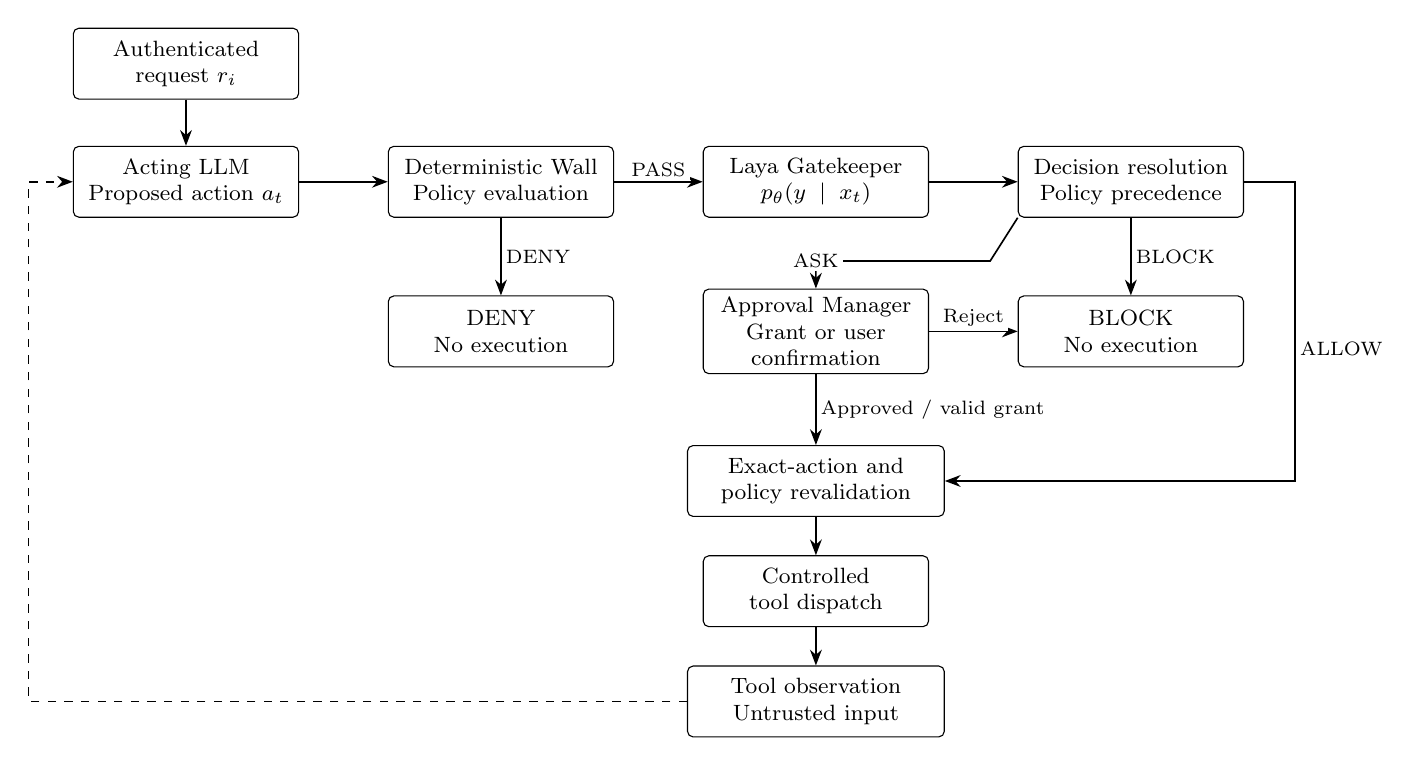
\begin{tikzpicture}

% Main authorization path
\node[pbox] (request) at (0,1.5)
{Authenticated request $r_i$};

\node[pbox] (agent) at (0,0)
{Acting LLM\\Proposed action $a_t$};

\node[pbox] (wall) at (4,0)
{Deterministic Wall\\Policy evaluation};

\node[pbox] (laya) at (8,0)
{Laya Gatekeeper\\$p_\theta(y\mid x_t)$};

\node[pbox] (router) at (12,0)
{Decision resolution\\Policy precedence};

% Decision outcomes
\node[pbox] (deny) at (4,-1.9)
{DENY\\No execution};

\node[pbox] (approval) at (8,-1.9)
{Approval Manager\\Grant or user confirmation};

\node[pbox] (blocked) at (12,-1.9)
{BLOCK\\No execution};

% Execution
\node[pwide] (recheck) at (8,-3.8)
{Exact-action and policy revalidation};

\node[pbox] (executor) at (8,-5.2)
{Controlled tool dispatch};

\node[pwide] (result) at (8,-6.6)
{Tool observation\\Untrusted input};

% Primary path
\draw[pedge] (request) -- (agent);
\draw[pedge] (agent) -- (wall);

\draw[pedge] (wall) --
node[plabel,above]{PASS} (laya);

\draw[pedge] (laya) -- (router);

% Wall denial
\draw[pedge] (wall) --
node[plabel,right]{DENY} (deny);

% BLOCK
\draw[pedge] (router) --
node[plabel,right]{BLOCK} (blocked);

% ASK
\draw[pedge]
(router.south west)
-- ++(-0.35,-0.55)
-| node[plabel,pos=0.7,above]{ASK}
(approval.north);

% ALLOW, routed outside the BLOCK node
\draw[pedge]
(router.east)
-- ++(0.65,0)
|- node[plabel,pos=0.28,right]{ALLOW}
(recheck.east);

% Approval outcomes
\draw[pedge] (approval.east) --
node[plabel,above]{Reject}
(blocked.west);

\draw[pedge] (approval.south) --
node[plabel,right]{Approved / valid grant}
(recheck.north);

% Tool execution
\draw[pedge] (recheck) -- (executor);
\draw[pedge] (executor) -- (result);

% Feedback to the next agent step
\draw[pedge,dashed]
(result.west)
-- (-2,-6.6)
-- (-2,0)
-- (agent.west);

\end{tikzpicture}%
}
\caption{Per-action authorization and execution.
The Wall enforces policy constraints before contextual
evaluation. The Gatekeeper's decision is resolved
subject to mandatory confirmation and grant validity.
Authorized actions undergo revalidation before dispatch.
Tool observations are returned as untrusted input.}
\label{fig:runtime}
\end{figure*}

% --------------------------------------------------
% 4.2 PERMISSION MEMORY
% --------------------------------------------------

\subsection{Permission Memory and Grant Lifecycle}

Permission memory maintains records of authenticated user decisions and reusable authorization grants. Its purpose is to preserve the scope of previous authorization rather than treating approval history as unrestricted permission.

We distinguish two mechanisms.

\textbf{1) Counting-based memory:}
The system records approvals associated with matching action patterns. Once a configurable threshold is reached, subsequent matching actions may be automatically approved. This mechanism serves as a baseline for studying the effects of repeated-approval learning. However, it can generalize one-time consent into reusable authority without an explicit standing grant. We therefore treat it as an experimental comparator rather than the preferred authorization mechanism.

\textbf{2) Explicit scoped grants:}
The current implementation maintains persistent,
user-specific grants in SQLite. Each grant binds
the exact tool, complete action arguments,
authentic user request, trusted contextual
facts, policy version, and tool schema.

The default grant lifetime is 86,400 seconds.
An optional maximum-use constraint limits
repeated execution. Grant reuse requires
validation of the recorded scope, expiry,
revocation status, and current authorization
state. Transactional usage reservations
prevent uncertain dispatch outcomes from
restoring consumed authorization.

An ordinary action approval does not establish
a reusable grant. Reusable authorization must
be issued separately through a trusted
authorization process. The current exact-scope
implementation does not support wildcard
or trust-class grants.


For a grant $g$, its validity is determined by:

\begin{equation}
\begin{split}
V(g,a_t,i,P^{(v)}) ={}&
I_{\mathrm{user}} \land I_{\mathrm{action}}\\
&\land I_{\mathrm{resource}}
\land I_{\mathrm{policy}}\\
&\land I_{\mathrm{expiry}}
\land I_{\mathrm{revocation}},
\end{split}
\end{equation}

where each indicator is true only when the corresponding identity, action, resource, policy version, expiry, or revocation condition is satisfied.

A grant is reusable only when:

\begin{equation}
V(g,a_t,i,P^{(v)})=1.
\end{equation}

A change in the applicable policy version invalidates grants tied to an earlier version unless they are explicitly revalidated. Revocation invalidates the corresponding exact-action grant. Broader class-scoped authorization and overlapping-grant revocation are not part of the current execution path.

Table~\ref{tab:memory_mechanisms} distinguishes one-time approval, explicit grant creation, and the counting-based experimental baseline.


\begin{table*}[!t]
\centering
\caption{Authorization reuse mechanisms and
their implementation status.}
\label{tab:memory_mechanisms}
\footnotesize
\begin{tabular}{p{3.2cm}p{7.0cm}p{5.0cm}}
\toprule
Mechanism & Authorization semantics & Status \\
\midrule
One-time approval &
Authorizes the exact pending action without
establishing reusable authority. &
Implemented approval path \\
\addlinespace
Exact scoped grant &
Permits reuse only when the authenticated user,
action binding, policy version, and grant
validity conditions match. &
Implemented with persistent SQLite state \\
\addlinespace
Counting-based reuse &
Automatically reuses matching approval patterns
after a configured threshold without requiring
a separate standing grant. &
Historical simulation baseline \\
\bottomrule
\end{tabular}
\end{table*}



Each memory record should preserve at least the following information:

\begin{itemize}
    \item Authenticated user and grant identifier.
    \item Tool name and permitted action or argument constraints.
    \item Exact resource identity and verified contextual constraints.
    \item Task scope, where the grant is task-specific.
    \item Applicable policy version.
    \item Issuance time, expiry time, and revocation status.
\end{itemize}


Grant records, learner state, feedback, and
audit information are maintained in persistent,
user-isolated storage. A pending tool invocation
is not automatically resumed after a restart.
Interactive standing-grant creation remains
an integration requirement, while broader
class-scoped grants belong to historical
simulation experiments rather than the
current exact-grant execution path.

% --------------------------------------------------
% 4.3 ADAPTIVE LEARNING
% --------------------------------------------------

\subsection{Adaptive Learning Mechanisms}

We investigate two complementary learning processes: per-user online adaptation of authorization decisions and periodic offline fine-tuning of the Gatekeeper model. These processes update different parameters and operate on different timescales.


\subsubsection{Per-User Contextual Learning}

The implemented contextual learner operates
above the frozen Gatekeeper and maintains
separate decision parameters for each user.
It estimates the cost of requesting
confirmation versus reusing an existing
exact-action grant.

The learner uses a 40-dimensional feature
representation comprising Gatekeeper
decision probabilities, grant age,
reviewed feedback counts, and encoded
trusted action characteristics. Let:

\begin{equation}
\boldsymbol{\phi}_t \in \mathbb{R}^{40}
\end{equation}

denote the contextual feature vector.
The learner maintains user-specific
parameters $\psi_i$ and applies a bounded
linear residual update using reviewed
feedback.

Its available actions are restricted to:

\begin{equation}
\mathcal{A}_t =
\begin{cases}
\{\Ask,\mathrm{USE\_GRANT}\}, & E_t=1,\\
\{\Ask\}, & E_t=0.
\end{cases}
\label{eq:bandit_actions}
\end{equation}

Here, $E_t=1$ indicates that the controller
has established eligibility for grant reuse.
This requires a Wall PASS, an eligible
Gatekeeper ASK, a valid exact-action grant,
complete required evidence, and the absence
of mandatory confirmation requirements.

The learner cannot authorize actions outside
this restricted decision space. Selecting
USE\_GRANT triggers revalidation of the
grant, action binding, and current policy
before execution. Ordinary approvals do
not independently create reusable authority.

The implemented learner uses a normalized
linear residual update with learning rate
0.05 and an exploration parameter of 0.1.
Its configured costs are 1 for requesting
confirmation, 0 for reviewed acceptable
reuse, and 10 for reviewed unwanted reuse.
Adaptive selection begins after 10 eligible
ASK observations.

The learner supports shadow operation,
in which recommendations are recorded
without authorizing execution, and active
operation within the controller's
enforcement constraints. The controlled
evaluation explicitly enables active
operation.

Alternative contextual algorithms, including
LinUCB, Linear Thompson Sampling, and
contextual epsilon-greedy, have also been
examined in historical offline simulations.
These variants are distinct from the bounded
linear cost learner used in the current
implementation. Their comparative behavior
under longer interaction histories and
changing user preferences remains a
research direction.


\subsubsection{Periodic Gatekeeper Fine-Tuning}

A proposed periodic adaptation process would
update the Gatekeeper's decision parameters
using independently verified feedback. Unlike contextual bandit learning, this process modifies the model itself.

Let $D_0$ denote the original supervised training dataset and $D_f$ the newly collected, independently verified feedback dataset. The updated model is trained using:

\begin{equation}
D_{\mathrm{train}} = D_0 \cup D_f.
\end{equation}

Initially, we propose freezing the encoder and fine-tuning only the decision heads. This reduces the number of trainable parameters and provides a controlled starting point for model adaptation.

The following techniques will be investigated:

\begin{itemize}

    \item \textbf{Experience replay:} Mix original training examples with verified feedback to reduce forgetting of previously learned authorization patterns.

    \item \textbf{Class-balanced sampling:} Prevent the updated model from becoming biased toward frequently observed approval categories.

    \item \textbf{Option-order shuffling:} Randomize the ordering of ALLOW, ASK, and BLOCK options during training to reduce sensitivity to label position.

    \item \textbf{Regularization:} Investigate methods such as Elastic Weight Consolidation to limit undesirable changes to previously learned parameters.

    \item \textbf{Probability calibration:} Evaluate temperature scaling and abstention-threshold fitting on a separate calibration dataset.

\end{itemize}

Raw user approvals are not directly treated as automatic training labels. Feedback must be evaluated against the original request, current policy, action scope, and actual outcome before it enters the training dataset. Shared-model updates must also account for user privacy and prevent individual authorization preferences from being indiscriminately transferred across users.

Each candidate checkpoint is evaluated against a frozen validation suite, held-out authorization examples, and prompt-injection regression cases. A checkpoint is deployed only if it satisfies predefined evaluation criteria. Otherwise, the previous checkpoint is retained.

Preference-based approaches such as RLHF, DPO, and KTO may be considered in future work, but their direct application to Laya's discriminative decision architecture requires separate investigation.

Figure~\ref{fig:learning} distinguishes the online per-user learning process from periodic model-level adaptation.



\begin{figure*}[!t]
\centering
\resizebox{0.97\textwidth}{!}{%
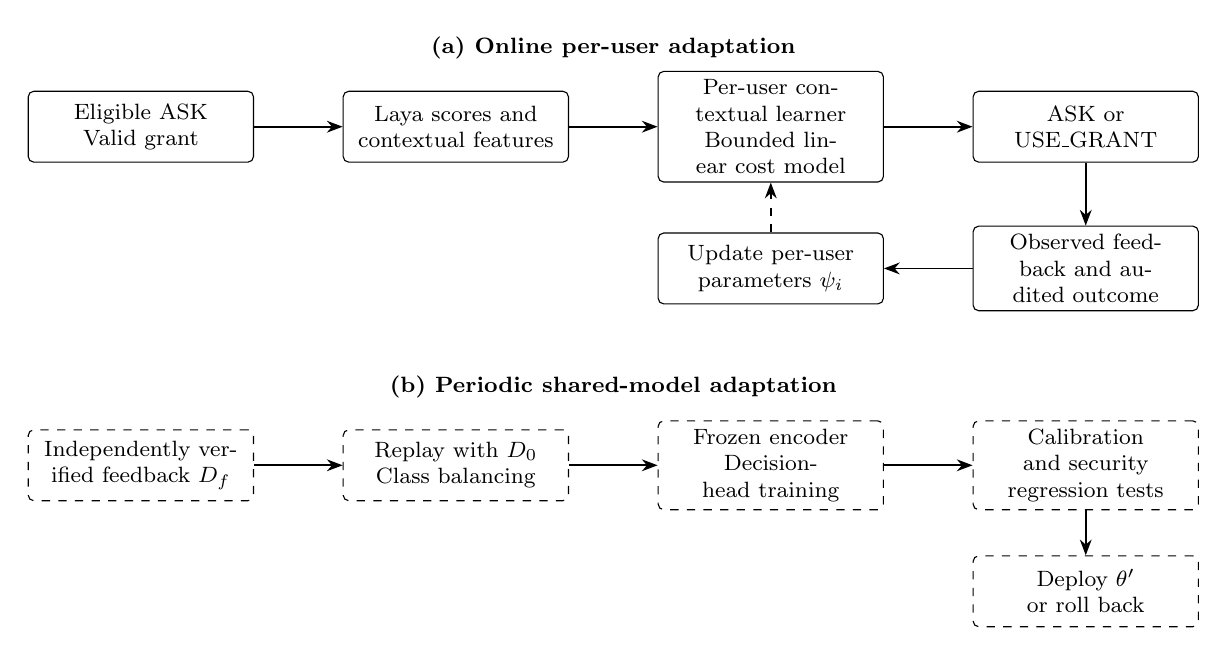
\begin{tikzpicture}

% ---------------------------------
% Online adaptation
% ---------------------------------

\node[font=\bfseries\footnotesize]
at (6,1.0)
{(a) Online per-user adaptation};

\node[pbox] (eligible) at (0,0)
{Eligible ASK\\Valid grant};

\node[pbox] (features) at (4,0)
{Laya scores and contextual features};

\node[pbox] (bandit) at (8,0)
{Per-user contextual learner\\
Bounded linear cost model};

\node[pbox] (choice) at (12,0)
{ASK or USE\_GRANT};

\node[pbox] (feedback) at (12,-1.8)
{Observed feedback and audited outcome};

\node[pbox] (update) at (8,-1.8)
{Update per-user parameters $\psi_i$};

\draw[pedge] (eligible) -- (features);
\draw[pedge] (features) -- (bandit);
\draw[pedge] (bandit) -- (choice);

\draw[pedge] (choice) -- (feedback);
\draw[pedge] (feedback) -- (update);

\draw[pedge,dashed]
(update.north) -- (bandit.south);

% ---------------------------------
% Periodic model adaptation
% ---------------------------------

\node[font=\bfseries\footnotesize]
at (6,-3.3)
{(b) Periodic shared-model adaptation};

\node[pplanned] (verified) at (0,-4.3)
{Independently verified feedback $D_f$};

\node[pplanned] (replay) at (4,-4.3)
{Replay with $D_0$\\Class balancing};

\node[pplanned] (training) at (8,-4.3)
{Frozen encoder\\Decision-head training};

\node[pplanned] (validation) at (12,-4.3)
{Calibration and security regression tests};

\node[pplanned] (deployment) at (12,-5.9)
{Deploy $\theta'$ or roll back};

\draw[pedge] (verified) -- (replay);
\draw[pedge] (replay) -- (training);
\draw[pedge] (training) -- (validation);
\draw[pedge] (validation) -- (deployment);

\end{tikzpicture}%
}
\caption{Implemented per-user contextual learning
and proposed periodic model adaptation.
The online learner updates user-specific
parameters while keeping Laya fixed.
The proposed offline process updates a shared
Gatekeeper checkpoint using verified feedback,
replay, calibration, and security validation.
Dashed nodes denote unimplemented extensions.}
\label{fig:learning}
\end{figure*}


% --------------------------------------------------
% 4.4 DECISION PRECEDENCE
% --------------------------------------------------

\subsection{Interfaces and Decision Precedence}
\label{sec:decision}

The authorization process must distinguish model predictions from the final execution decision. We define the Wall verdict as:

\begin{equation}
W(P_i^{(v)},a_t,c_t)\in\{\Pass,\Deny\}.
\end{equation}

The Gatekeeper returns:

\begin{equation}
\mathbf{p}_t =
(p_A,p_Q,p_B),
\end{equation}

where the three entries correspond to \Allow, \Ask, and \Block.

Let $m_t$ indicate whether confirmation is mandatory, $k_t$ indicate whether critical evidence is complete, and $g_{i,t}$ indicate whether a valid explicit grant matches the proposed action.

The decision policy follows this precedence:

\begin{equation}
d_t =
\begin{cases}
\Block, & B_t=1,\\
\Ask, & M_t=1,\\
\Allow, & A_t=1,\\
\Allow, & U_t=1,\\
\Ask, & \text{otherwise}.
\end{cases}
\label{eq:final_decision}
\end{equation}

Here, $B_t=1$ denotes a Wall denial, invalid
action binding, or Gatekeeper BLOCK condition,
including $\hat y_t=\Block$ or $p_B\geq\tau_B$.
The indicator $M_t=1$ denotes
$m_t=1$ or $k_t=0$, representing mandatory
confirmation or incomplete critical evidence.

The indicator $A_t=1$ requires
$\hat y_t=\Allow$ and $p_A\geq\tau_A$.
Finally, $U_t=1$ requires $E_t=1$,
a USE\_GRANT selection by the contextual
learner, and successful revalidation of
the exact-action grant and current policy.

The conditions are evaluated in the
precedence order shown in
(\ref{eq:final_decision}).

The model prediction is
$\hat y_t=\arg\max_y p_\theta(y\mid x_t)$.
The eligibility conditions represented by
$E_t$ are established through trusted
controller checks described in
Section~\ref{sec:architecture}; they do not
depend on an unimplemented ASK-reason
classifier.

Before execution, the controller computes an action binding over the authenticated user, task, canonical action arguments, resource, and policy version:

\begin{equation}
b_t =
H(i,\mathrm{task}_i,a_t,\rho_t,P_i^{(v)}),
\end{equation}

where $H$ is a cryptographic hash over the canonical representation. The executor rechecks this binding and the current policy before dispatch. Any change to the relevant action or authorization state invalidates the previous decision.

\begin{algorithm}[!htbp]
\footnotesize
\caption{Runtime Authorization of a Proposed Tool Action}
\label{alg:runtime}
\begin{algorithmic}[1]
\Require User request $r_i$, action $a_t$, context $c_t$, policy $P_i^{(v)}$
\Require Gatekeeper $f_\theta$, grant memory, user policy $\pi_{\psi_i}$
\Ensure Final authorization decision $d_t$

\If{action schema or binding is invalid}
    \State \Return $\Block$
\EndIf

\If{$W(P_i^{(v)},a_t,c_t)=\Deny$}
    \State \Return $\Block$
\EndIf

\State $p_t \gets f_\theta(r_i,a_t,c_t,P_i^{(v)})$
\State $\hat y_t \gets \arg\max_y p_t(y)$

\If{$\hat y_t=\Block$ \textbf{or}
    $p_t(\Block)\geq\tau_B$}
    \State \Return $\Block$
\EndIf

\If{$m_t=1$ \textbf{or} $k_t=0$}
    \State \Return $\Ask$
\EndIf

\If{$\hat y_t=\Allow$ \textbf{and} $p_t(\Allow)\geq\tau_A$}
    \State \Return $\Allow$
\EndIf

\If{$\hat y_t\neq\Ask$}
    \State \Return $\Ask$
\EndIf

\If{$E_t\neq 1$}
    \State \Return $\Ask$
\EndIf

\State $u_t \gets \pi_{\psi_i}(x_t,\{\Ask,\mathrm{USE\_GRANT}\})$

\If{$u_t=\mathrm{USE\_GRANT}$}
    \If{grant and action binding remain valid}
       \State \Return $\Allow$
    \EndIf
\EndIf
\State \Return $\Ask$

\end{algorithmic}
\end{algorithm}


% --------------------------------------------------
% 4.5 DESIGN TRADEOFFS AND IMPLEMENTATION STATUS
% --------------------------------------------------

\subsection{Design Tradeoffs and Implementation Status}

The architecture separates policy enforcement, model inference, and adaptive authorization because these components have different update requirements. The Wall is changed only through an authenticated policy-update process. User-specific bandit parameters can be updated during interactions, whereas the shared Gatekeeper model is updated only through a separate, validated training cycle.

This separation also introduces practical tradeoffs. More restrictive grant scopes reduce the possibility of unintended permission reuse but may increase confirmation frequency. Broader trust-class grants may reduce interruptions but require stronger scope validation and revocation handling. Similarly, contextual bandit adaptation can reduce repeated confirmation requests, but its effectiveness depends on the reliability of feedback and the reward definition. Fine-tuning may improve general decision quality, but introduces risks of overfitting, forgetting, and transfer of user-specific behavior into a shared checkpoint.


The current implementation includes deterministic
policy enforcement, Laya-based contextual
assessment, persistent exact-action grants,
a bounded per-user contextual learner, and
controlled permission evaluation.

Permission records, feedback, learner state,
and audit information are maintained in SQLite.
The controller validates action bindings and
authorization state before tool dispatch.
The learner supports shadow operation and
active evaluation within the deterministic
permission boundary.

The implemented learner differs from the
LinUCB and Thompson Sampling variants
examined in historical offline experiments.
Periodic fine-tuning of Laya using verified
authorization feedback has not yet been
demonstrated. Complete interactive approval
handling, independent label adjudication,
and broader end-to-end benchmark evaluation
remain necessary.


% ==========================================
% V. EXPERIMENTAL METHODOLOGY
% ==========================================

\section{Experimental Methodology}
\label{sec:methodology}

\subsection{Evaluation Design}

We evaluate three aspects of the authorization
framework: permission reuse under controlled
action sequences, Gatekeeper classification
against provisional reference labels, and
real-model controller integration.

The controlled evaluation exercises the
authorization controller, deterministic Wall,
persistent grant mechanism, and contextual
learner using constructed scenarios and
simulated tool execution.

The Gatekeeper evaluation separately measures
agreement between released Laya checkpoints
and a fixed authorization dataset. The
integration check examines whether actual
Laya predictions are correctly handled by
the controller.

These experiments evaluate different system
components and are not treated as equivalent
measurements of end-to-end agent security.

\subsection{Controlled Permission Scenarios}

The controlled evaluation includes Workspace,
Slack, and Banking scenarios. The dataset
contains 36 constructed action sequences,
with 14 action checks per sequence.

Each experimental configuration therefore
processes 504 action checks.

The scenarios use scripted user preferences,
constructed authorization states, and
simulated tool execution. The evaluation
does not involve human participants or
complete autonomous agent trajectories.

\subsection{Experimental Configurations}

We compare three authorization configurations.

\textbf{No memory:}
The controller processes authorization requests
without adaptive permission reuse.

\textbf{Explicit grants:}
The controller reuses authenticated exact-action
grants when their scope, policy version,
expiry, and revocation conditions remain valid.

\textbf{Active contextual learner:}
The controller additionally enables the
implemented user-specific bounded contextual
cost learner. The learner selects between
requesting confirmation and reusing an
existing valid grant.

All configurations retain deterministic
policy enforcement.

\subsection{Gatekeeper Evaluation}

A separate evaluation compares recorded Laya
checkpoint and question configurations on
150 authorization examples.

The examples are distributed equally across
the provisional ALLOW, ASK, and BLOCK labels.

Because these labels have not undergone
complete independent human adjudication,
we report agreement with provisional labels
rather than validated classification accuracy.

A further 12-case CPU-based evaluation
examines actual Laya inference and the
resulting controller decisions.

\subsection{Evaluation Metrics}

We report confirmation requests, authorized
dispatches, forbidden dispatches under the
scenario oracle, and agreement with
provisional authorization labels.

Confirmation reduction is defined as:

\begin{equation}
R_k =
\frac{Q_0-Q_k}{Q_0},
\label{eq:confirmation_reduction}
\end{equation}

where $Q_0$ is the number of confirmation
requests without memory and $Q_k$ is the
corresponding count for configuration $k$.

Forbidden dispatches are determined using
the constructed scenario oracle. A zero
count therefore indicates compliance with
the evaluated scenarios, not a universal
security guarantee.

% ==========================================
% VI. EXPERIMENTAL RESULTS
% ==========================================

\section{Experimental Results}
\label{sec:results}

\subsection{Controlled Permission Evaluation}

Table~\ref{tab:permission_results} compares
the three permission configurations over
504 action checks each.

\begin{table}[!t]
\centering
\caption{Controlled permission evaluation
($N=504$ per configuration).}
\label{tab:permission_results}
\footnotesize
\setlength{\tabcolsep}{3pt}
\begin{tabular}{lrrr}
\toprule
Configuration & ASK & Dispatch & Forbidden \\
\midrule
No memory       & 168 & 168 & 0 \\
Explicit grants & 139 & 197 & 0 \\
Active learner  & 159 & 177 & 0 \\
\bottomrule
\end{tabular}
\end{table}

Relative to the no-memory baseline,
explicit grants reduce confirmation requests
by 17.26\%, corresponding to 29 fewer
requests. The active contextual learner
reduces requests by 5.36\%, corresponding
to nine fewer requests.

All three configurations record zero
forbidden dispatches under the constructed
scenario oracle.

Explicit grants produce the largest
confirmation reduction in this evaluation.
The active learner does not outperform
deterministic grant reuse, indicating that
online adaptation does not necessarily
provide additional short-term efficiency.

These findings are limited to the
constructed scenarios and should not
be interpreted as end-to-end agent
task-completion or attack-prevention results.

\subsection{Gatekeeper Classification Results}

Table~\ref{tab:laya_results} reports
agreement with the provisional labels
of the 150-example authorization dataset.

\begin{table}[!t]
\centering
\caption{Laya agreement with provisional
authorization labels ($N=150$).}
\label{tab:laya_results}
\footnotesize
\setlength{\tabcolsep}{4pt}
\begin{tabular}{lrr}
\toprule
Configuration & Agreement & Rate (\%) \\
\midrule
Base historical    & 48/150 & 32.00 \\
Typed baseline     & 54/150 & 36.00 \\
Typed decomposed   & 53/150 & 35.33 \\
Cybersec baseline  & 66/150 & 44.00 \\
Cybersec rotated   & 70/150 & 46.67 \\
\bottomrule
\end{tabular}
\end{table}

The Cybersec rotated configuration achieves
the highest recorded agreement at 46.67\%,
compared with 44.00\% for the corresponding
Cybersec baseline.

However, agreement alone does not establish
authorization safety. False approvals may
have substantially greater consequences
than unnecessary confirmations or false
blocks.

The comparison also includes different
checkpoint and question configurations.
Accordingly, the results do not establish
improvements from project-specific model
fine-tuning.

Independent label adjudication and
risk-sensitive evaluation are required
before drawing stronger conclusions
about Gatekeeper reliability.

\subsection{Real-Model Integration}

A separate CPU-based integration check
evaluates 12 authorization cases using
the pinned base Laya checkpoint.

All 12 inference requests complete without
recorded errors. The final controller
decisions agree with the expected outcomes
in 10 cases, corresponding to 83.33\%.

Agreement is 3/3 for expected ALLOW,
4/6 for ASK, and 3/3 for BLOCK.

The two disagreements involve expected
ASK decisions that are classified as BLOCK.

This small evaluation demonstrates limited
real-model controller integration but does
not establish general authorization accuracy
or performance under complete agent
trajectories.

% ==========================================
% VII. DISCUSSION, LIMITATIONS, AND FUTURE WORK
% ==========================================

\section{Discussion, Limitations, and Future Work}

\subsection{Security and Authorization Tradeoffs}

The proposed framework separates deterministic policy enforcement from contextual authorization and feedback-driven adaptation. This separation establishes an important distinction between an action that satisfies explicit permission constraints and one that is appropriate for the user's current task. The Wall enforces the former, while the Gatekeeper evaluates the latter. Consequently, the effectiveness of the combined system depends on both the completeness of the underlying policy and the reliability of contextual decision inference.

The deterministic enforcement boundary prevents learning components from overriding explicitly prohibited actions. However, this property does not guarantee that every action permitted by the Wall is consistent with user intent. Broadly defined permissions may still admit unintended operations, while an imperfect Gatekeeper may incorrectly classify actions that satisfy the deterministic policy. The proposed architecture therefore does not eliminate the security--utility tradeoff. Instead, it provides independently enforceable constraints within which contextual decision-making can be evaluated and improved.

The use of a lightweight decision model introduces a further tradeoff between inference efficiency and authorization quality. Replacing repeated generative evaluations with structured classification may reduce computational overhead, but this advantage depends on model latency, input preparation costs, and the frequency of additional confirmation requests. A faster classifier that produces excessive false blocks or unnecessary ASK decisions may reduce overall task utility. Accordingly, computational efficiency must be evaluated jointly with authorization accuracy and legitimate task completion rather than through model inference time alone.

\subsection{Adaptive Authorization and Permission Creep}

Approval learning introduces a separate challenge: reducing repeated user confirmations without treating previous consent as unrestricted future authority. Counting-based permission memory can reduce interruptions by automatically reusing frequently approved action patterns. However, such reuse may incorrectly generalize authorization across resources, tasks, or execution contexts.

Explicit scoped grants provide a more controlled alternative by separating approval of an individual action from authorization of future actions. Nevertheless, the security of this mechanism depends on the precision of grant matching, the handling of broader resource classes, and the correctness of expiration and revocation procedures. A valid grant must not bypass mandatory confirmation, compensate for missing task evidence, or override a Gatekeeper BLOCK.


The controlled evaluation shows that adaptive
learning does not necessarily improve upon
explicit grant reuse. Although both mechanisms
reduce confirmation requests relative to the
no-memory baseline, deterministic grant reuse
produces the larger reduction in the tested
scenarios.

The active learner's additional conservatism
and dependence on reviewed feedback may
limit its short-term confirmation savings.
Whether contextual learning provides greater
benefits under longer interaction histories,
changing preferences, or more heterogeneous
tasks remains unresolved.


An additional difficulty arises from partial feedback. User responses are directly observable primarily when confirmation is requested, while automatically authorized actions may provide only indirect execution outcomes. Furthermore, an approval does not establish that an action was objectively safe or that confirmation was unnecessary. These properties require careful reward design, conservative exploration, and evaluation using independently verified authorization outcomes.

\subsection{Limitations and Threats to Validity}

The current implementation and evaluation have several limitations.

First, the permission-classification datasets contain labels reviewed primarily through language-model-based procedures rather than independent human adjudication. Disagreements between source labels and subsequent reviews indicate that authorization criteria must be applied consistently before classifier accuracy can be interpreted as a reliable measure of decision quality.

Second, the effectiveness of the Gatekeeper depends on the information available at inference time. Context compaction addresses model input-length constraints, but it may omit evidence relevant to particular authorization decisions. Furthermore, the live controller does not yet expose all historical tool observations and trusted identity information available in offline evaluation. This creates a potential discrepancy between the model's evaluated inputs and its operational inputs.

Third, the controlled permission evaluation
uses constructed action sequences, scripted
preferences, and simulated tool execution.
Although the implemented authorization
controller and persistent permission mechanisms
are exercised, these experiments do not
establish performance under authentic human
approval behavior or complete agent trajectories.

Fourth, the per-user contextual learner has
been implemented and evaluated, but its
observed confirmation reduction is smaller
than that achieved by explicit grants alone.
The experiments do not establish long-term
adaptation benefits. Periodic fine-tuning
of the shared Gatekeeper remains unevaluated,
and the available model-comparison labels
have not undergone complete independent
human adjudication.

Finally, the security properties of the framework assume complete mediation of tool execution, correct resource identification, authenticated approval records, and integrity of the policy enforcement components. Compromise of these trusted components or errors in the original permission policy fall outside the guarantees provided by the proposed learning mechanisms.

\subsection{Future Research Directions}

Future work will investigate three primary directions.

\textbf{1) Extended contextual learning:}
Building on the implemented bounded contextual
learner, we will compare LinUCB, Linear
Thompson Sampling, and conservative exploration
under longer interaction histories and
changing user preferences. The evaluation will
examine confirmation reduction, unsafe grant
reuse, adaptation speed, and robustness to
incomplete or unreliable feedback. Offline
policy evaluation will precede any deployment
of learned automatic authorization behavior.

\textbf{2) Continual Gatekeeper adaptation:}
We will investigate periodic fine-tuning of Laya's decision heads using independently verified authorization feedback. Experience replay, class-balanced sampling, option-order shuffling, and probability calibration will be evaluated to determine whether incremental training improves contextual classification without degrading previously learned behavior. Candidate checkpoints will undergo held-out authorization evaluation and prompt-injection regression testing before deployment. More extensive model adaptation will be considered only if decision-head updates prove insufficient.

\textbf{3) Long-term authorization consistency:}
We will investigate interactive grant issuance,
revocation behavior, long-term storage correctness,
and cross-session authorization consistency.
Particular attention will be given to preventing
authorization transfer across unrelated tasks,
resources, and users. Evaluation will also
examine how policy changes and conflicting
feedback affect previously learned preferences.

A broader evaluation will compare deterministic enforcement, contextual authorization, explicit grants, and adaptive learning under matched multi-step agent workloads. AgentDojo \cite{debenedetti2024agentdojo} provides a basis for measuring task completion and prompt-injection attack success. Additional action-level annotations and longitudinal approval scenarios will be necessary to evaluate authorization accuracy, permission creep, and confirmation behavior directly.


% ==========================================
% VIII. CONCLUSION
% ==========================================

\section{Conclusion}

This paper presents a policy-bounded authorization architecture for tool-using LLM agents that separates deterministic permission enforcement, contextual action evaluation, and adaptive approval management. The framework evaluates proposed tool invocations throughout an agent's execution trajectory rather than relying solely on permissions established at task initiation. A deterministic Wall constrains executable actions, while a lightweight Gatekeeper provides structured ALLOW, ASK, and BLOCK assessments based on the user request and relevant execution context.


Controlled evaluation across 504 action
checks per configuration shows that explicit
grants reduce confirmation requests by
17.26\%, compared with 5.36\% for the
active contextual learner. All three
configurations record zero forbidden
dispatches under the scenario oracle.

These results support the feasibility of
policy-bounded permission reuse but do not
establish an advantage for contextual learning
over deterministic grants in the evaluated
setting. Separate Gatekeeper comparisons
highlight the need for independently
validated authorization labels and
risk-sensitive classification metrics.

Future evaluation will examine longer
interaction histories, real-user feedback,
end-to-end agent workloads, and periodic
model adaptation to determine whether
authorization quality and confirmation
efficiency can be improved without
expanding user-granted authority.



% ==========================================
% REFERENCES
% ==========================================

\begin{thebibliography}{00}

\bibitem{debenedetti2024agentdojo}
E. Debenedetti, J. Zhang, M. Balunovi\'c,
L. Beurer-Kellner, M. Fischer, and F. Tram\`er,
``AgentDojo: A Dynamic Environment to Evaluate
Prompt Injection Attacks and Defenses for LLM Agents,''
in \emph{Advances in Neural Information Processing Systems},
vol. 37, 2024.
[Online]. Available:
\url{https://arxiv.org/abs/2406.13352}.

\bibitem{shi2025progent}
T. Shi, J. He, Z. Wang, L. Wu, H. Li, W. Guo,
and D. Song,
``Progent: Programmable Privilege Control for LLM Agents,''
arXiv:2504.11703, 2025.
[Online]. Available:
\url{https://arxiv.org/abs/2504.11703}.

\bibitem{tsai2025conseca}
L. Tsai and E. Bagdasaryan,
``Contextual Agent Security: A Policy for Every Purpose,''
in \emph{Proceedings of the Workshop on Hot Topics
in Operating Systems (HotOS)}, 2025,
doi: 10.1145/3713082.3730378.

\bibitem{zhu2025miniscope}
J. Zhu, K. Tseng, G. Vernik, X. Huang,
S. G. Patil, V. Fang, and R. A. Popa,
``MiniScope: A Least Privilege Framework for
Authorizing Tool Calling Agents,''
arXiv:2512.11147, 2025.
[Online]. Available:
\url{https://arxiv.org/abs/2512.11147}.

\bibitem{sequeira2026agentsentry}
R. Sequeira, S. Damianakis, U. Iqbal,
and K. Psounis,
``Agent-Sentry: Bounding LLM Agents via
Execution Provenance,''
arXiv:2603.22868, 2026.
[Online]. Available:
\url{https://arxiv.org/abs/2603.22868}.

\bibitem{tu2026tasklp}
A. Tu and M. Tu,
``Task-Conditioned Least-Privilege Learning for
Executable Terminal and MCP Agents,''
arXiv:2608.18351, 2026.
[Online]. Available:
\url{https://arxiv.org/abs/2608.18351}.

\bibitem{wu2026skillscope}
J. Wu, Y. Nan, Y. Lin, H. Wang, Y. Xiao,
S. Wang, and Z. Zheng,
``SkillScope: Toward Fine-Grained Least-Privilege
Enforcement for Agent Skills,''
arXiv:2605.05868, 2026.
[Online]. Available:
\url{https://arxiv.org/abs/2605.05868}.

\bibitem{li2010contextualbandit}
L. Li, W. Chu, J. Langford, and R. E. Schapire,
``A Contextual-Bandit Approach to Personalized
News Article Recommendation,''
in \emph{Proceedings of the 19th International
Conference on World Wide Web}, 2010,
pp. 661--670,
doi: 10.1145/1772690.1772758.

\bibitem{shu2026agentcl}
Y. Shu, B. Jim\'enez Guti\'errez,
S. P. Jonnalagedda, Y. Yao, H. Sun,
and Y. Su,
``AgentCL: Toward Rigorous Evaluation of
Continual Learning in Language Agents,''
arXiv:2606.02461, 2026.
[Online]. Available:
\url{https://arxiv.org/abs/2606.02461}.

\bibitem{zhang2026consistencygate}
Y. Zhang and S. Li,
``ConsistencyGate: Preventing Memory Contamination
in LLM Agents via Self-Consistency Admission Control,''
arXiv:2607.22962, 2026.
[Online]. Available:
\url{https://arxiv.org/abs/2607.22962}.

\end{thebibliography}

\end{document}